\newpage
\section{Analysis} \label{analysis}

For implementaiton of the methods introduced in previous section the SVAR package in R \footcite[See.][]{Lange2020} software is used.
\subsection{Transitions Channels}
In Figure on can see a general plot of changes in the variables introduecd in .
\begin{figure}[H]
\caption{Interest Rate, Government Spending and House Price in Germany in Years 2000-2020}
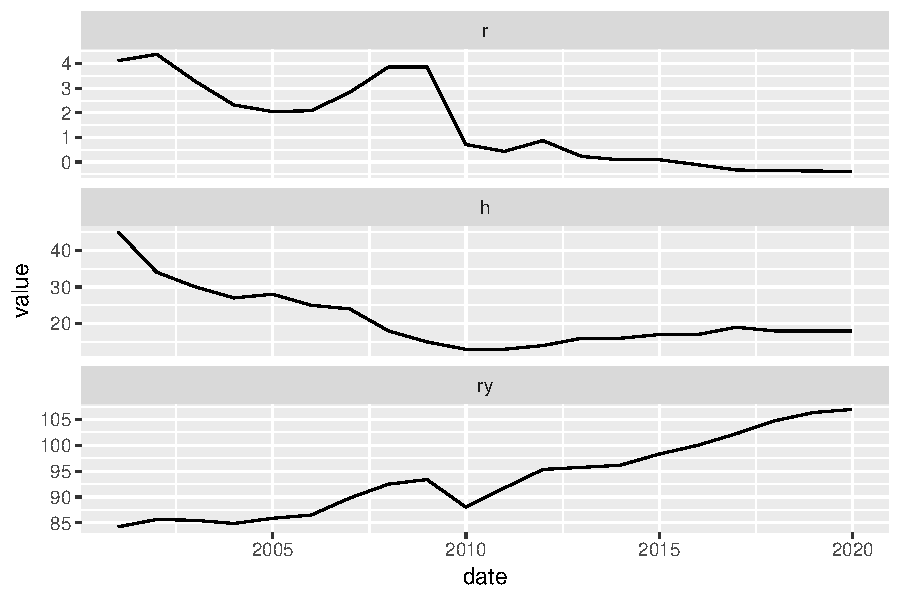
\includegraphics[width=0.9\textwidth]{interestRateOnOutput}
\\
\cite[Quelle: Own Graph][]{FOM}
\end{figure}

As one can see a has lead to house price to decrease.

\subsection{SVAR}
The following picture shows the results of the identified model to different schocks
\begin{figure}[H]
\caption{Interest Rate, Government Spending and House Price in Germany in Years 2000-2020}
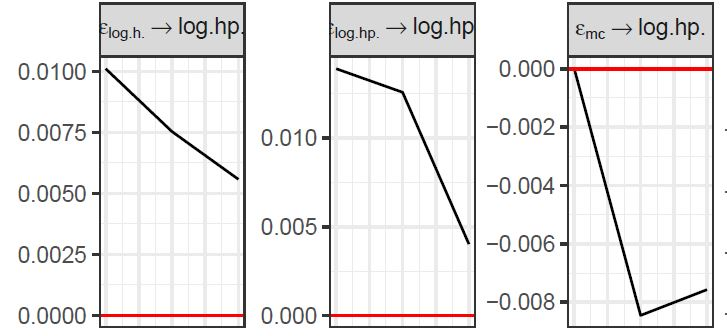
\includegraphics[width=0.9\textwidth]{hp1}
\\
\cite[Quelle: Own Graph][]{FOM}
\end{figure}
\begin{figure}[H]
\caption{Interest Rate, Government Spending and House Price in Germany in Years 2000-2020}
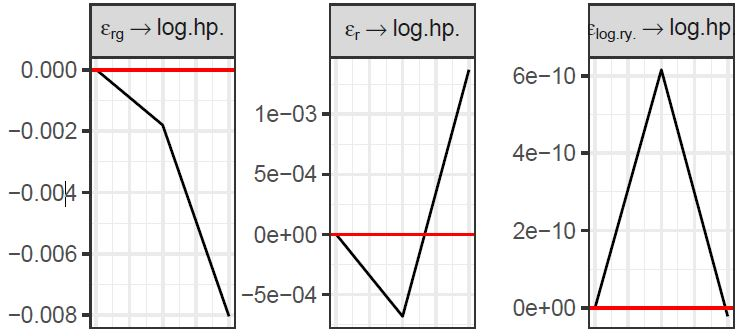
\includegraphics[width=0.9\textwidth]{hp2}
\\
\cite[Quelle: Own Graph][]{FOM}
\end{figure}


